\documentclass[12pt,a4paper]{article}
\usepackage[legalpaper, portrait, lmargin=1cm, rmargin=1cm, tmargin=2cm, bmargin=2cm]{geometry}
\usepackage{fancyhdr}
\usepackage{amsmath}
\usepackage{amssymb}
\usepackage{graphicx}
\usepackage{wrapfig}
\usepackage{blindtext}
\usepackage{hyperref}
\usepackage{pdflscape}
\usepackage{svg}
\usepackage[most]{tcolorbox}
\usepackage{xcolor}

\graphicspath{ {./} }

\definecolor{linkcolor}{HTML}{1588e0}

\hypersetup{
  colorlinks=true,
  allcolors=linkcolor,
  pdftitle={Relatório AMS - Entrega 2 - 2022/2023},
  pdfpagemode=FullScreen,
}

\definecolor{bg}{rgb}{1,0.96,0.9}

\pagestyle{fancy}
\fancyhf{}
\rhead{Grupo \textbf{37}}
\lhead{Relatório Entrega 2 AMS 2022/2023 LEIC-A}
\cfoot{Diogo Gaspar (99207), Diogo Correia (99211) e Tiago Silva (99335)}

\renewcommand{\footrulewidth}{0.2pt}

\renewcommand{\labelitemii}{$\circ$}
\renewcommand{\labelitemiii}{$\diamond$}


\begin{document}
\begin{titlepage}
  \begin{center}
    \vspace*{5cm}

    \Huge
    \textbf{Projeto AMS - Entrega 2}

    \vspace{0.5cm}
    \LARGE
    Grupo 037 | Turno L08 | LEIC-A

    \vspace{0.5cm}
    \large
    Prof. Maria do Rosário Carvalho

    \vfill
  \end{center}
  \large
  \begin{itemize}
    \item[] \textbf{Diogo Gaspar} (99207) - 14h
    \item[] \textbf{Diogo Correia} (99211) - 14h
    \item[] \textbf{Tiago Silva} (99335) - 14h
  \end{itemize}
\end{titlepage}

\begin{tcolorbox}[enhanced jigsaw,colback=bg,boxrule=0pt,arc=4pt]
  \begin{large}
    \textbf{Notas:}
  \end{large}

  \begin{small}
    \textbf{(B.1.) Integração dos modelos da "Vista de Negócio"} (Figures \ref{fig:archimate}, \ref{fig:p-set-bpmn} \& \ref{fig:p-on-bpmn})
  \end{small}
  \begin{itemize}
    \item TODO
  \end{itemize}

  \begin{small}
    \textbf{(B.2.) Diagramas de Casos de Uso} (Figures \ref{fig:uc-run} \& \ref{fig:uc-store})
  \end{small}
  \begin{itemize}
    \item TODO
  \end{itemize}

  \begin{small}
    \textbf{(B.3.) Diagrama de Classes (em UML) do modelo de domínio} (Figure \ref{fig:uml})
  \end{small}
  \begin{itemize}
    \item TODO
  \end{itemize}

  \begin{small}
    \textbf{(B.4.) Diagrama de Máquina de Estados} (Figure \ref{fig:state-machine})
  \end{small}
  \begin{itemize}
    \item TODO
  \end{itemize}

  \begin{small}
    \textbf{(B.5.) Diagrama de Blocos} (Figure \ref{fig:bbd})
  \end{small}
  \begin{itemize}
    \item TODO
  \end{itemize}

  \begin{small}
    \textbf{(B.6.) Diagrama Interno de Blocos} (Figure \ref{fig:ibd})
  \end{small}
  \begin{itemize}
    \item TODO
  \end{itemize}
\end{tcolorbox}

\begin{landscape}
  \begin{figure}
    \centering
    \includesvg[inkscapelatex=false,width=1.5\textwidth]{assets/archimate.svg}
    \caption{(B.1.) Diagrama de Vista Geral do Negócio}
    \label{fig:archimate}
  \end{figure}
\end{landscape}

\begin{landscape}
  \begin{figure}
    \centering
    \includesvg[inkscapelatex=false,width=1.5\textwidth]{assets/p_set.svg}
    \caption{(B.1.) Diagrama do Processo P-SET}
    \label{fig:p-set-bpmn}
  \end{figure}
\end{landscape}

\begin{landscape}
  \begin{figure}
    \centering
    \includesvg[inkscapelatex=false,width=1.35\textwidth]{assets/p_on.svg}
    \caption{(B.1.) Diagrama do Processo P-ON}
    \label{fig:p-on-bpmn}
  \end{figure}
\end{landscape}

\begin{landscape}
  \begin{figure}
    \centering
    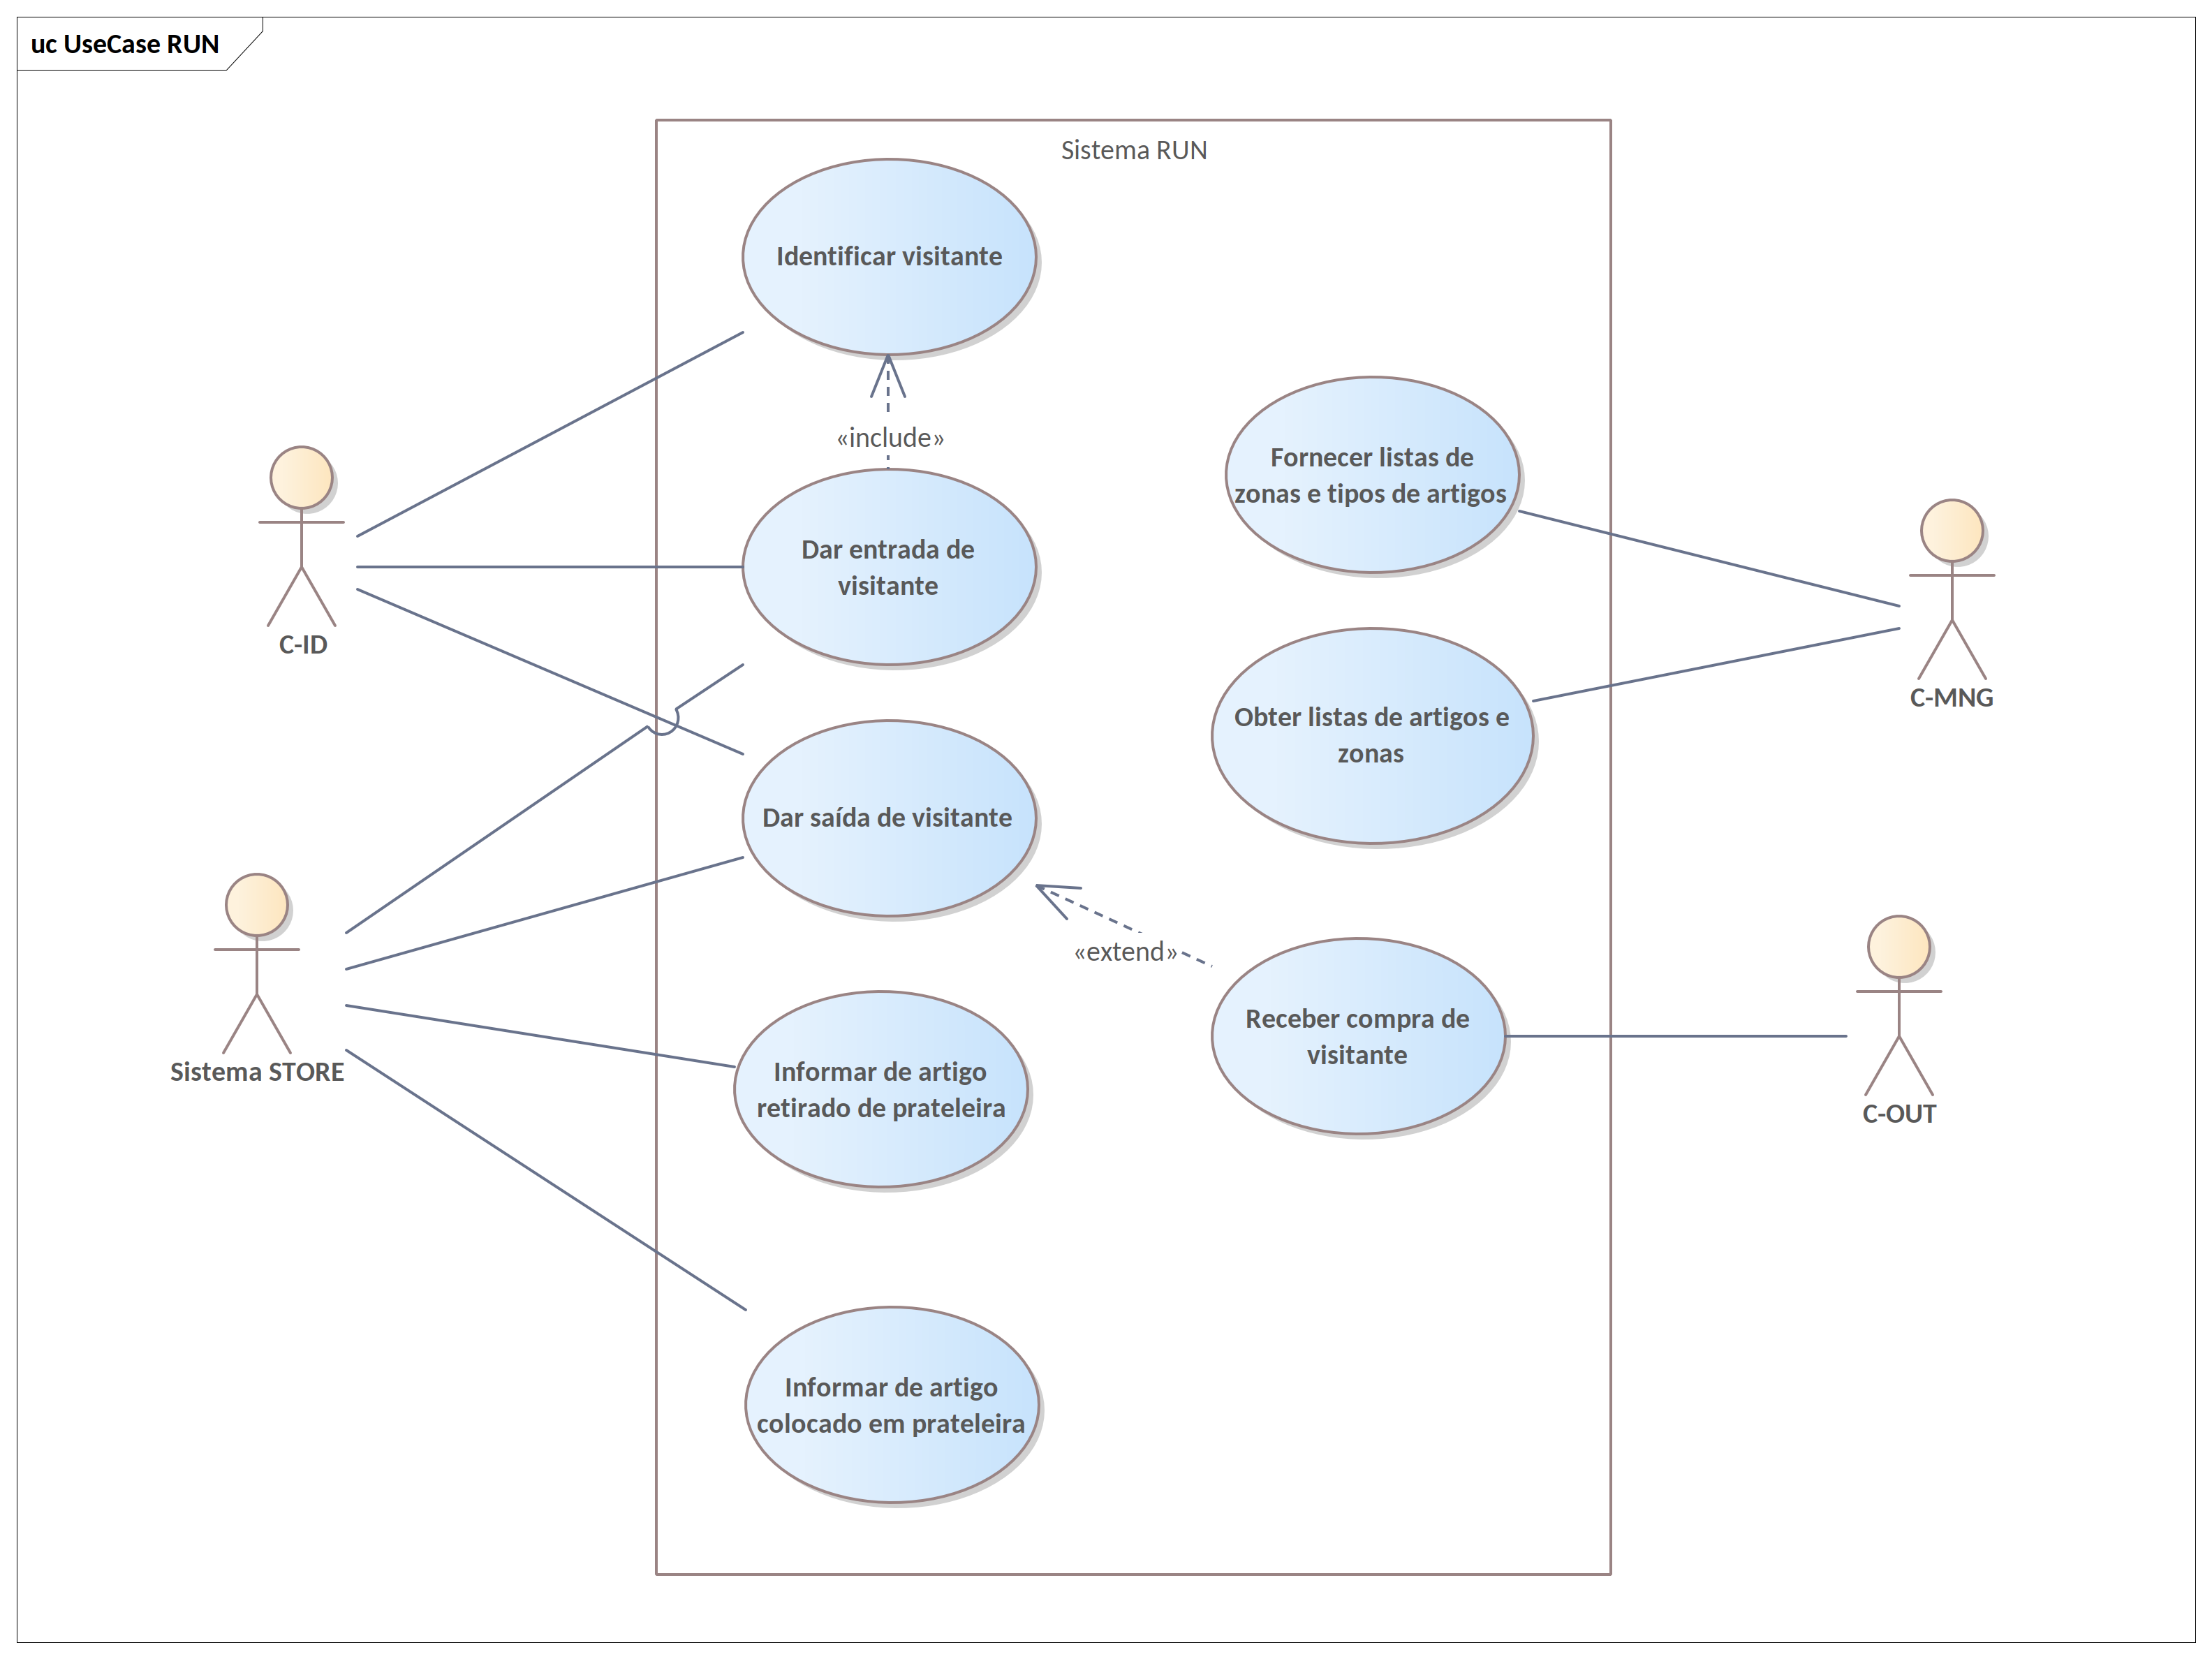
\includegraphics[width=1.3\textwidth]{assets/ea-usecase-run.png}
    \caption{(B.2.) Diagrama de Casos de Uso do sistema RUN}
    \label{fig:uc-run}
  \end{figure}
\end{landscape}

\begin{landscape}
  \begin{figure}
    \centering
    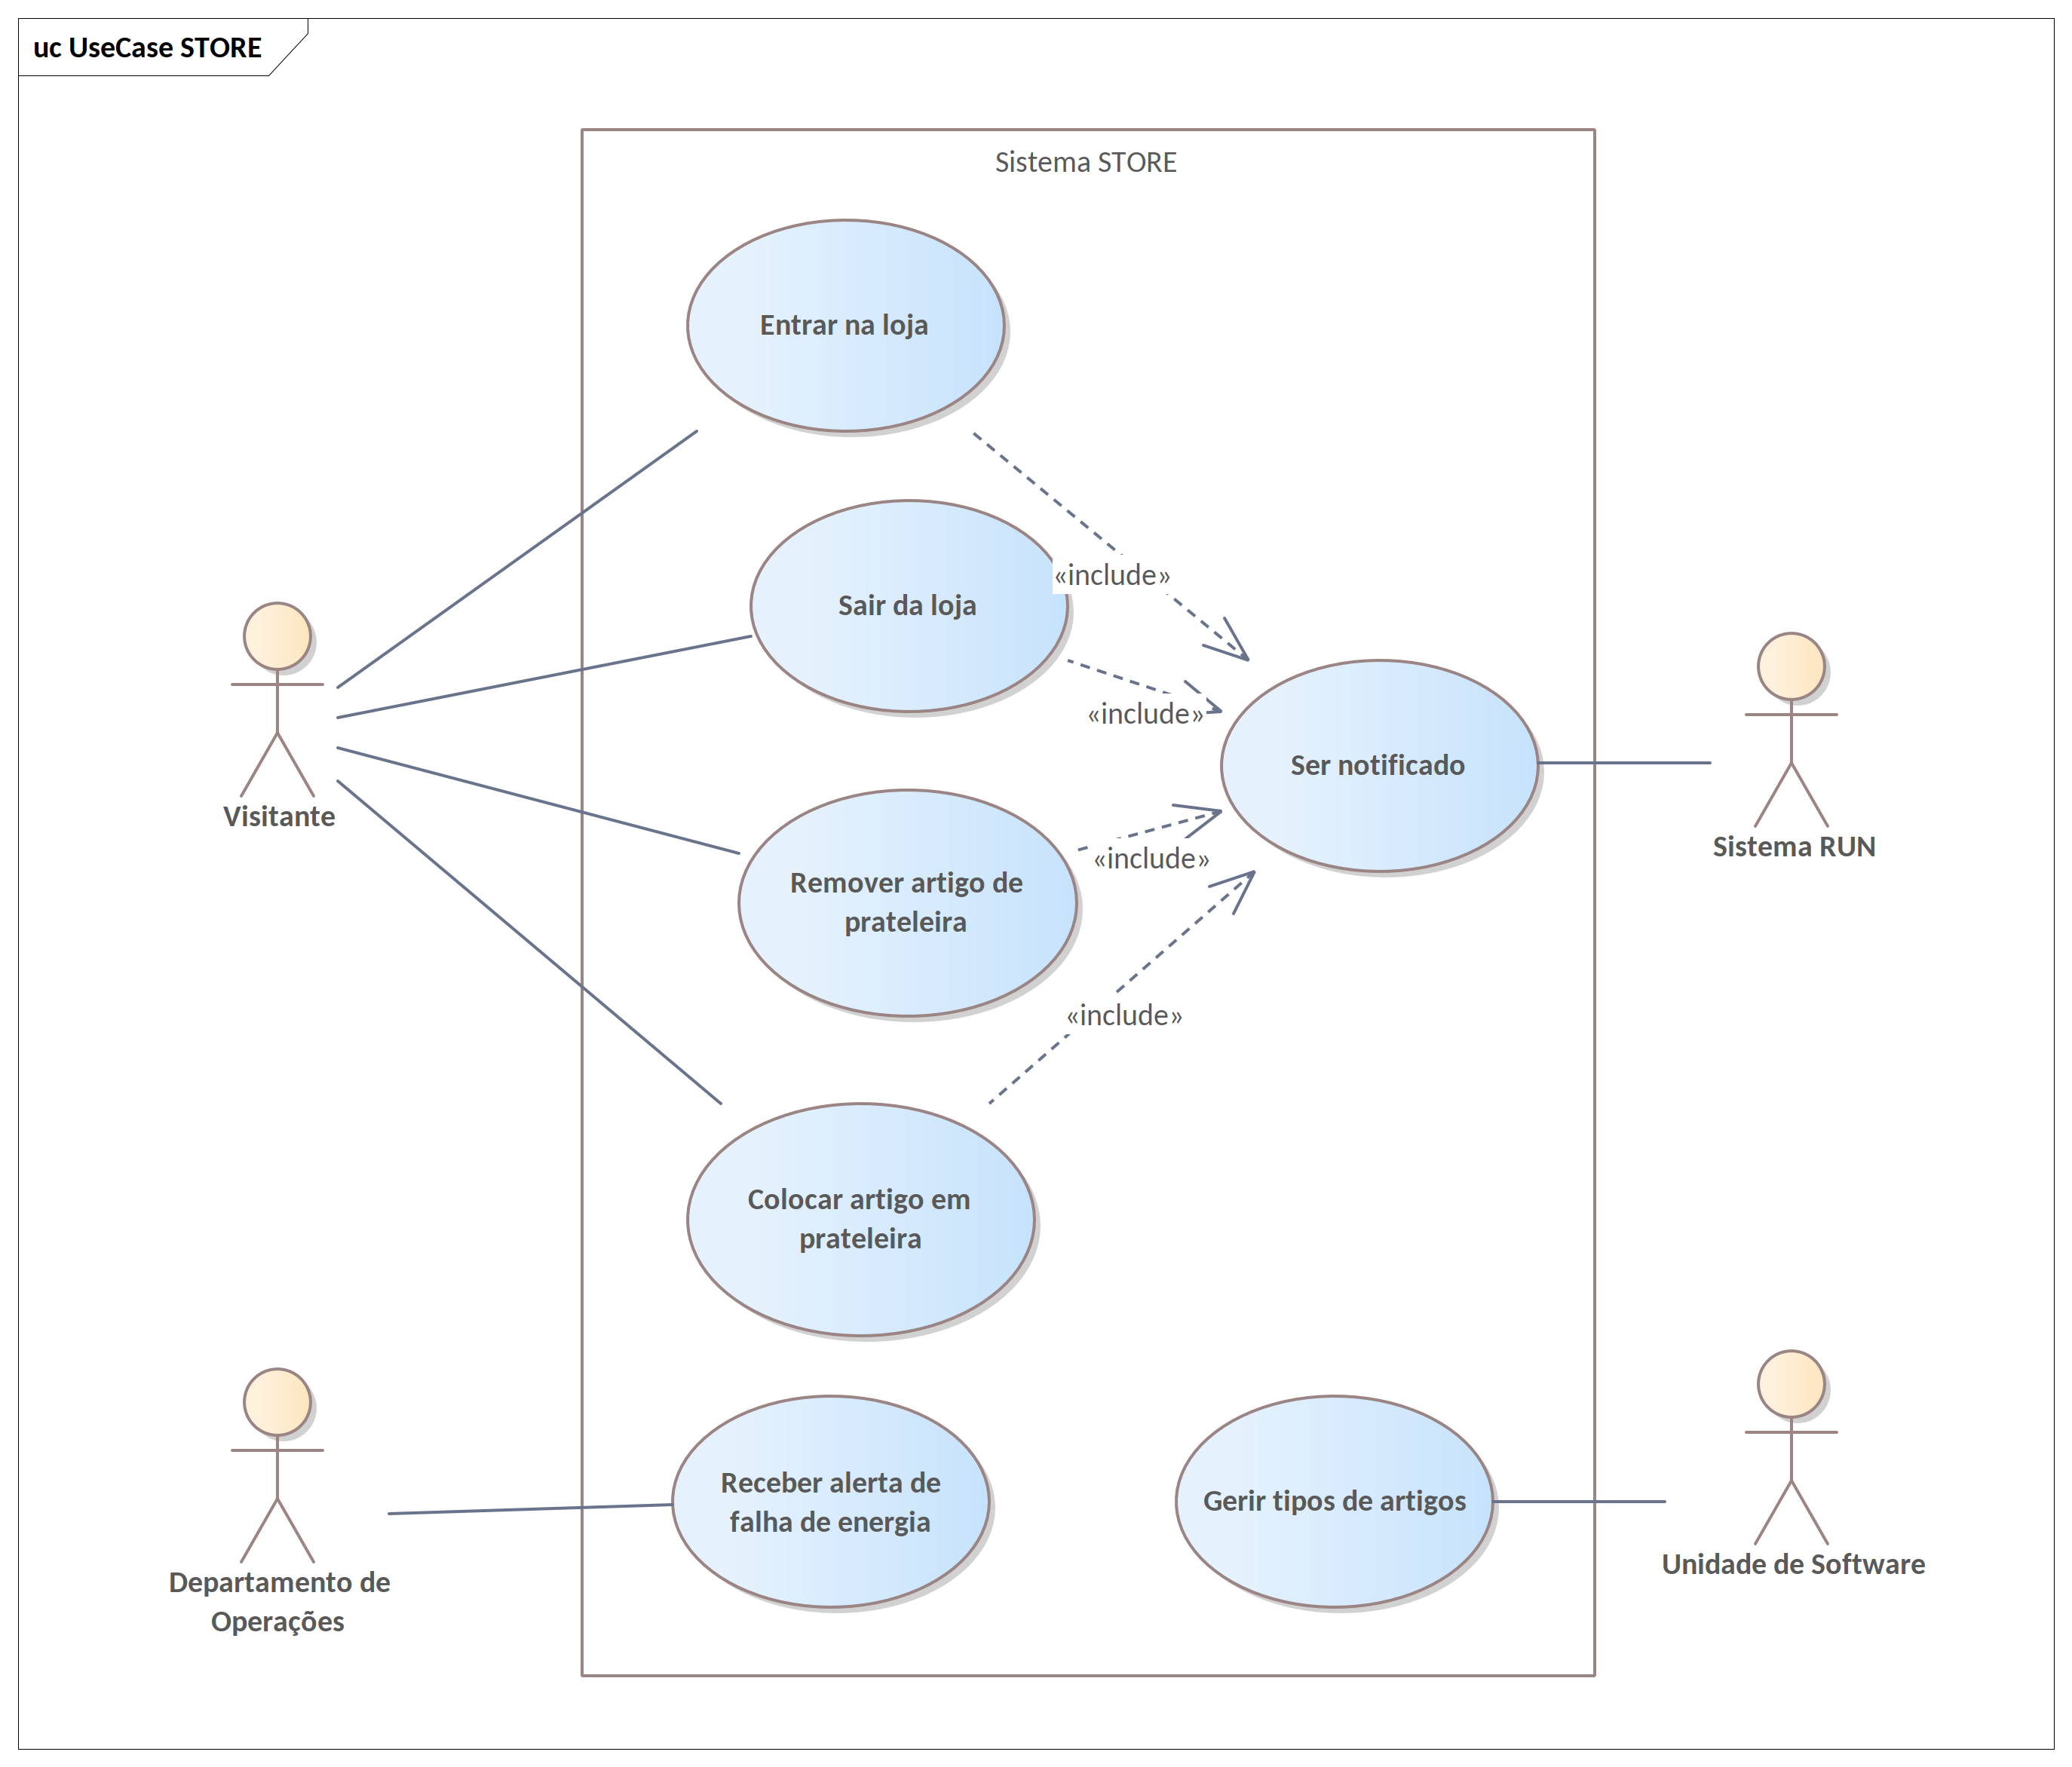
\includegraphics[width=1.15\textwidth]{assets/ea-usecase-store.png}
    \caption{(B.2.) Diagrama de Casos de Uso do sistema STORE}
    \label{fig:uc-store}
  \end{figure}
\end{landscape}

\begin{landscape}
  \begin{figure}
    \centering
    \includesvg[inkscapelatex=false,width=1.35\textwidth]{assets/p_on.svg}
    \caption{(B.3.) Diagrama de Classes (em UML) do modelo de domínio}
    \label{fig:uml}
  \end{figure}
\end{landscape}

\begin{landscape}
  \begin{figure}
    \centering
    \includesvg[inkscapelatex=false,width=1.35\textwidth]{assets/p_on.svg}
    \caption{(B.4.) Diagrama de Máquina de Estados}
    \label{fig:state-machine}
  \end{figure}
\end{landscape}

\begin{landscape}
  \begin{figure}
    \centering
    \includesvg[inkscapelatex=false,width=1.35\textwidth]{assets/p_on.svg}
    \caption{(B.5.) Diagrama de Blocos}
    \label{fig:bbd}
  \end{figure}
\end{landscape}

\begin{landscape}
  \begin{figure}
    \centering
    \includesvg[inkscapelatex=false,width=1.35\textwidth]{assets/p_on.svg}
    \caption{(B.6. Diagrama Interno de Blocos)}
    \label{fig:ibd}
  \end{figure}
\end{landscape}

\end{document}